%% bare_jrnl.tex — revised with embedded TODOs
%% =====================================================================
%% MASTER TODO LIST
%% =====================================================================
%% [HIGH]  T01. Compute Diebold–Mariano statistics (Table VI) and fill in.
%% [HIGH]  T02. Recompute all QLIKE summary statistics with the variance
%%               floor and replace the placeholder numbers in the abstract,
%%               Table V, §V.A, §VI.A, and §VII.
%% [HIGH]  T03. Recompute MEDIAN QLIKE values (currently placeholders in
%%               Table V).
%% [HIGH]  T04. Verify the HMM-filter acceptance rate. The current text
%%               claims 100% acceptance — this must be computed, not asserted.
%% [HIGH]  T05. Generate the three figures (fig_vol_forecast,
%%               fig_forecast_errors, fig_val_errors) and place the PDFs
%%               in the same directory as the .tex file.
%% [HIGH]  T06. Compute the Monte-Carlo bias correction for the
%%               maturity-aligned E[log] plug-in (see §III.D TODO) and
%%               add a paragraph to §V.D reporting the bias estimate.
%% [HIGH]  T07. Verify all remaining references exist. Removed refs are
%%               listed in the revision note; do NOT re-add refs you cannot
%%               verify online.
%% [MED]   T08. Add the empirical justification for the rolling-volatility
%%               dominance finding in §VII.A (the paragraph currently says
%%               "consistent with two features" — add a diagnostic figure
%%               or a short table if possible).
%% [MED]   T09. Decide whether to keep or cut §IV.C (the HMM discussion);
%%               currently states "100% acceptance" — if true, consider
%%               moving to a footnote, since the contribution is zero.
%% [MED]   T10. Cross-check the reported trade counts in Table VIII — the
%%               totals were computed from unrounded source values and may
%%               differ by ±0.01 from the displayed component sums.
%% [LOW]   T11. Add line numbers to the .tex file if the target journal
%%               requires them (use \usepackage{lineno} + \linenumbers).
%% [LOW]   T12. Add ORCID iDs to the author block if available.
%% [LOW]   T13. Check that the abstract is ≤ 250 words and keywords
%%               are alphabetized (IEEE style).
%% [LOW]   T14. Run a spell-check pass with aspell or hunspell.
%% [LOW]   T15. Verify the SHA-256 checksums in §IV.B against the actual
%%               dataset files on disk.
%% =====================================================================

\documentclass[journal]{IEEEtran}

\usepackage{cite}
\usepackage{graphicx}
\usepackage{amsmath}
\usepackage{amssymb}
\usepackage{array}
\usepackage{tabularx}
\usepackage{booktabs}
\usepackage{float}
\usepackage{hyperref}

\hyphenation{op-tical net-works semi-conduc-tor}

\begin{document}

\title{EGARCH Volatility Forecasting and Maturity-Aligned Pricing for NIFTY~50 Index Options: An Empirical Evaluation}

\author{
\IEEEauthorblockN{Heet Kothari, Meet Mehta, Shaurya Jain, Pramod Bide}
\IEEEauthorblockA{}
}
% TODO [T12 - LOW]: Add ORCID iDs and affiliations, e.g.
%   \IEEEauthorblockA{Dept.~of Computer Engineering, XYZ Institute, Mumbai, India\\
%   Email: \{heet.kothari, meet.mehta, ...\}@xyz.edu}

\markboth{}%
{Kothari \MakeLowercase{\textit{et al.}}: EGARCH Forecasting and Maturity-Aligned Option Pricing on NIFTY~50}

\maketitle

\begin{abstract}
% TODO [T02 - HIGH]: The QLIKE values in this abstract are placeholders.
% After re-running the pipeline with the variance floor, replace the
% italicised placeholder values below with the actual computed numbers.
% Also verify that the abstract is ≤ 250 words.
% TODO [T13 - LOW]: Verify abstract word count.
We evaluate three distinct empirical questions on NIFTY~50 data from July~2024 to December~2025: (i)~a walk-forward comparison of rolling volatility, GARCH(1,1), and EGARCH(1,1,1); (ii)~a Black--Scholes valuation comparison using rolling, one-step EGARCH, and maturity-aligned EGARCH variance inputs on 189{,}084 historical option observations; and (iii)~a small deterministic daily-options backtest. On the common 312-observation forecast sample, rolling volatility achieves the lowest MAE (0.068347) and EGARCH the highest (0.082915); EGARCH's variance QLIKE is dominated by near-zero forecasts and must be interpreted with a variance floor. In valuation, maturity-aligned EGARCH improves over one-step EGARCH but does not beat the rolling benchmark in any moneyness or maturity group. The backtest produces only 13 strategy-level trades, and HMM-filtered EMA trades exactly duplicate unfiltered EMA trades; no profitability claim is made. All option prices are last-traded daily CLOSE references, not executable bid--ask quotes. The principal empirical contribution is a transparent demonstration that short-window historical volatility is a difficult benchmark to beat for one-step forecasting and for constant-maturity BSM inputs on this sample.
\end{abstract}

\begin{IEEEkeywords}
% TODO [T13 - LOW]: Alphabetise the keywords (IEEE style).
NIFTY~50, option valuation, Black--Scholes, volatility forecasting, GARCH, EGARCH, maturity-aligned variance, walk-forward evaluation.
\end{IEEEkeywords}

\IEEEpeerreviewmaketitle

\section{Introduction}

Volatility estimation is central to derivative valuation: an option's value depends on the uncertainty expected over its remaining life. The relevant horizon is therefore important—a one-day volatility forecast describes the next observation period, whereas an option with several weeks to maturity depends on accumulated uncertainty across many future trading days.

The Black--Scholes--Merton (BSM) framework provides an analytical benchmark for European option valuation \cite{black1973,merton1973}, but requires a volatility input treated as constant. Daily financial returns exhibit time-varying conditional variance. The ARCH and GARCH families model this dependence through functions of past innovations and conditional variances \cite{engle1982,bollerslev1986}. EGARCH expresses conditional variance in log form and permits asymmetric responses to positive and negative innovations \cite{nelson1991}. These properties motivate a comparison of rolling historical volatility, GARCH(1,1), and EGARCH(1,1,1) with $(p,o,q)=(1,1,1)$; asymmetric structure does not, however, imply superior out-of-sample forecasting.

Using a volatility forecast rather than the contract's contemporaneous implied volatility avoids using the same market premium both to infer and to evaluate a volatility input. The resulting BSM value remains conditional on model assumptions and is not an independently observed fair value.

The study therefore compares one-step EGARCH volatility with a maturity-aligned variance formed by aggregating daily forecasts over the remaining trading horizon. The implemented construction is a deterministic expected-log-variance plug-in approximation, not an exact analytical multi-step EGARCH solution. Volatility forecast accuracy and option-price valuation error are consequently treated as distinct empirical objectives.

Hidden Markov Models (HMMs) provide probabilistic state models for sequences with latent states \cite{rabiner1989,hamilton1994}. In this study, two-state and three-state HMM fits are used as diagnostics only, while a separate causal two-state HMM is used to filter EMA signals in the daily-options backtest. The HMM is not an input to the BSM valuation experiment, and changing transition matrices across diagnostic fits do not establish stable regimes or predictive superiority.

The empirical gap addressed here is narrowly defined: how do one-day volatility forecast comparisons relate to maturity-aligned volatility inputs in historical BSM valuation, and what descriptive outcomes arise from a separate daily-options backtest under explicit daily-bar execution assumptions? The experiments use a chronological NIFTY~50 setting from July~2024 to December~2025. The index dataset contains 375 daily observations from Yahoo Finance (\texttt{\string^NSEI}); the options dataset contains 605{,}159 normalized records across 375 dates from NSE daily F\&O bhavcopy files. These sources are distinct, and the available option data do not include historical bid--ask quotes, intraday candles or timestamps, historical implied volatility, or order-book depth. Daily option CLOSE is therefore a last-traded reference price rather than an executable bid--ask quote.

\subsection*{Contributions}

\begin{itemize}
\item \textbf{Chronological volatility forecast comparison:} a walk-forward comparison of rolling historical volatility, GARCH(1,1), and EGARCH(1,1,1) using daily NIFTY~50 returns, with Diebold--Mariano tests on the common evaluation sample.
% TODO [T01 - HIGH]: The DM tests must actually be reported in Table VI.
% Once computed, uncomment the sentence below with the actual direction
% and significance of the results.
% (Placeholder) The DM comparisons do not reject equal predictive accuracy
% at the 5% level for any pair, consistent with the short sample size.
\item \textbf{Maturity-aligned option valuation:} an empirical comparison of rolling, one-step EGARCH, and maturity-aligned EGARCH inputs in the BSM model on 189{,}084 historical NSE option closing references.
\item \textbf{Transparent daily-options backtesting:} a chronological exercise with explicit next-session entries, option-specific risk management, and daily-bar exits, reported without any profitability claim.
\item \textbf{Evidence-based limitations:} clear reporting of data availability, execution assumptions, and the boundaries of interpretation.
\end{itemize}

\subsection*{Research Questions}

\begin{enumerate}
\item \textbf{RQ1:} How do rolling volatility, GARCH(1,1), and EGARCH(1,1,1) compare in forecasting the next-day volatility of NIFTY~50 returns under chronological evaluation?
\item \textbf{RQ2:} How does maturity-aligned EGARCH variance, relative to one-step EGARCH and rolling volatility, change Black--Scholes pricing deviations for daily NIFTY~50 options across option types, moneyness, and maturity ranges?
\item \textbf{RQ3:} What descriptive outcomes and limitations arise when deterministic daily-options strategies are evaluated under the specified entry, exit, and risk-management assumptions?
\item \textbf{RQ4:} Does the causal two-state HMM filter materially alter EMA signal selection or trade outcomes, and does the available test sample support any claim of improvement?
\end{enumerate}

The remainder of the paper is organized as follows. Section~II reviews related work. Section~III describes data and methodology. Section~IV documents implementation and reproducibility. Section~V presents results, Section~VI discusses findings and limitations, and Section~VII concludes and outlines future work.

\section{Related Work}

\subsection{Option Pricing and the Black--Scholes--Merton Framework}

Black and Scholes established a closed-form framework for European option valuation under continuous trading, frictionless markets, and constant-volatility diffusion \cite{black1973}. Merton extended it to account for dividends and related issues \cite{merton1973}. We use BSM as a transparent valuation benchmark, not as a claim that its assumptions hold exactly for NIFTY~50 options.

Implied volatility is obtained by inverting a pricing model against an observed price. It reflects risk premia, supply and demand, liquidity, discrete dividends, and model conventions; the volatility smile and skew indicate that a single constant volatility does not fit all strikes and maturities equally well. Stochastic-volatility models (Heston \cite{heston1993}) and local-volatility approaches (Dupire \cite{dupire1994}) provide important extensions; the SABR framework and its implied-volatility approximation \cite{sabr2002} provide another influential treatment of smile risk. We do not empirically implement these models; we instead use BSM with volatility inputs generated from historical forecasting models.

\subsection{Conditional Volatility Modeling}

Engle modelled conditional variance as a function of past squared innovations \cite{engle1982}. Bollerslev's GARCH formulation adds lagged conditional variance and provides a parsimonious representation of volatility persistence \cite{bollerslev1986}. Nelson's EGARCH expresses conditional variance in log form and permits asymmetric response to shocks without imposing non-negativity constraints \cite{nelson1991}. GARCH(1,1) is consequently a natural benchmark for daily NIFTY~50 volatility forecasting, and asymmetric EGARCH(1,1) is a natural comparison because equity-index returns are commonly characterized by volatility clustering and asymmetric shock responses. We do not treat EGARCH as superior a priori.

\subsection{Volatility Forecast Evaluation}

Volatility forecasts should be evaluated chronologically so that model fitting uses only information available before each forecast date; expanding-window or walk-forward procedures are preferable to random partitioning. Forecast conditional volatility is the model-generated quantity, whereas the realized proxy is the observable or constructed quantity used to evaluate that forecast. A one-day conditional-volatility forecast is not automatically an appropriate constant input for an option with several weeks to maturity; a maturity-aligned approximation must aggregate or otherwise map the daily forecast to the remaining option horizon.

We use mean absolute error (MAE) and root mean squared error (RMSE) as scale-dependent summaries of forecast accuracy. QLIKE is a loss function for evaluating variance forecasts; its interpretation depends on how the realized variance proxy and forecast variance are defined and matched by date and horizon. The Diebold--Mariano test compares predictive accuracy through the time series of loss differentials \cite{diebold_mariano}; its use requires common forecast dates, a common target and horizon, an explicitly stated loss function, and appropriate treatment of serial correlation.

\subsection{Hidden Markov Models and Financial Regimes}

An HMM represents a sequence of observations through an unobserved discrete state process, state-dependent emission distributions, and transition probabilities. Rabiner provides a foundational treatment of HMM inference and estimation \cite{rabiner1989}; Hamilton develops the application of regime-switching models to economic time series \cite{hamilton1994}. For financial applications, causal regime estimation requires a distinction between filtered and smoothed probabilities: a filtered probability at date $t$ may use observations through $t$, whereas a smoothed probability can use later observations and is unsuitable for a real-time trading decision.

\subsection{Research Gap and Motivation}

The literature provides established tools for three linked but distinct tasks. Conditional-volatility models supply forecasts that can be evaluated against a daily volatility target. Option-pricing theory supplies a common framework for translating those forecasts into theoretical prices. Regime models provide a causal state estimate that can be used to filter a deterministic trading rule. These tasks should be assessed separately because forecasting accuracy, option-pricing accuracy, detection of price deviations, and realized trading profitability are not interchangeable outcomes.

\section{Data and Methodology}

\subsection{Research Design}

The study contains three related but distinct empirical components. First, daily NIFTY~50 returns are used to evaluate rolling, GARCH, and asymmetric EGARCH volatility forecasts. Second, historical NIFTY~50 option records are valued with the continuous-dividend BSM model using alternative historical volatility inputs. Third, a separate deterministic daily-options backtest evaluates technical trading rules under explicit contract-selection and execution conventions. The backtest is not an integrated execution of the EGARCH--BSM valuation pipeline; the HMM is used to filter EMA signals in the backtest and is not a volatility input to the BSM valuation experiment.

\subsection{Data Sources and Preprocessing}

The index dataset was obtained from the Yahoo Finance chart API for \texttt{\string^NSEI}. It contains daily OHLC observations from 1 July 2024 through 31 December 2025, comprising 375 observations. The options dataset consists of normalized NSE daily F\&O bhavcopy records over the same period: 605,159 records for CE and PE contracts, including daily OHLC fields, expiry, strike, contracts, open interest, settlement, and related source fields. The experiments thus combine NSE options data with third-party Yahoo Finance index data.

Dates are parsed and sorted before alignment. Duplicate index dates are removed, while duplicate option contract-date groups are checked using trade date, expiry, strike, and option type. Decimal log returns are computed from consecutive index closing prices as
\begin{equation}
r_t=\ln\left(\frac{C_t}{C_{t-1}}\right),
\end{equation}
where $C_t$ is the NIFTY~50 closing price. Positive \texttt{contracts} are required for eligible valuation and execution observations, and valuation records also require a positive option CLOSE. Zero-volume records remain in the source dataset but are excluded from these eligible observations. Records with zero settlement are retained as a diagnostic issue rather than being universally removed. Calendar days-to-expiry (DTE) are used for option eligibility, whereas observed NIFTY trading dates are used when aggregating future variances.

\subsection{Volatility Target and Forecasting Models}

The evaluated next-day volatility proxy is the annualized absolute log return,
\begin{equation}
\sigma^{\mathrm{target}}_{t+1}=\left|r_{t+1}\right|\sqrt{252}.
\end{equation}
This is a one-day realized proxy based on the next closing-price return; it is not an intraday realized-variance estimator or a direct observation of latent volatility.

The rolling benchmark is the sample standard deviation of the most recent 20 returns with \texttt{ddof=1}, annualized by $\sqrt{252}$. An EWMA benchmark is also evaluated with $\lambda=0.94$. The GARCH benchmark uses a constant mean, normal innovations, and $(p,o,q)=(1,0,1)$. Both conditional-volatility models use an expanding historical estimation window with a minimum of 60 observations and produce one-step forecasts. For EGARCH we use constant mean, normal innovations, $(p,o,q)=(1,1,1)$, and returns multiplied by 100 before fitting; the conditional log variance under the \texttt{arch} parameterization is
\begin{equation}
\log(\sigma_t^2)=\omega+\alpha_1\left(\left|e_{t-1}\right|-\sqrt{\frac{2}{\pi}}\right)+\gamma_1 e_{t-1}+\beta_1\log(\sigma_{t-1}^2),
\qquad e_t=\frac{\epsilon_t}{\sigma_t}.
\end{equation}
Here $\omega$ is the log-variance intercept, $\alpha_1$ measures the response to shock magnitude, $\gamma_1$ captures signed-shock asymmetry, and $\beta_1$ measures log-variance persistence. Forecast variance on the percentage scale is divided by $10{,}000$ to obtain decimal daily variance; taking its square root gives decimal daily volatility, and multiplying by $\sqrt{252}$ gives annualized volatility. Walk-forward fits with nonzero convergence flags or invalid forecasts are recorded as failures and are not replaced with synthetic values.

\subsection{Maturity-Aligned Variance Construction}

% TODO [T06 - HIGH]: The current recursion is an E[log] plug-in and is a
% Jensen-type LOWER BOUND on the true multi-step conditional variance.
% Add a short Monte-Carlo validation paragraph here (or in §V.D) that
% quantifies the bias on the training residuals:
%
%   1. Fit EGARCH on the training window.
%   2. Simulate M = 10,000 paths of length N from the fitted EGARCH.
%   3. Compute the mean of the N-step summed variance across paths.
%   4. Compare this Monte-Carlo estimate to the plug-in approximation
%      for the same initial state and horizon.
%   5. Report the ratio MC / plug-in (typically 1.0 – 1.5 depending on
%      alpha_1 and gamma_1).
%
% Alternatively, if the arch package version you use exposes
% `model.forecast(horizon=N)` for EGARCH, replace the plug-in with the
% analytical multi-step forecast and DELETE the Jensen paragraph below.
For an option with $N$ observed NIFTY trading dates through expiry, the first daily percentage-scale variance is the analytical one-step EGARCH forecast. Because the employed library interface does not expose analytical multi-step EGARCH forecasts in the original implementation, later values were originally propagated deterministically. The present version replaces that plug-in with a controlled approximation and we distinguish it explicitly from the exact conditional expectation. For $h\ge 2$,
\begin{equation}
\widehat h^{(\%)}_{t+h}=\exp\left(\omega+\beta_1\log\widehat h^{(\%)}_{t+h-1}\right),
\end{equation}
which ignores the $\alpha_1$- and $\gamma_1$-weighted innovation contributions in expectation. Because $E[\exp(X)]\neq\exp(E[X])$ in general, the resulting multi-step variance is a Jensen-type lower bound on the analytical multi-step conditional variance. We therefore report it as an \emph{expected-log-variance plug-in} and quantify the bias with a Monte-Carlo comparison on the training residuals (see §V.D). The values are converted to decimal daily variances by $\widehat v_{t+h}=\widehat h^{(\%)}_{t+h}/10{,}000$. The maturity-aligned annualized volatility is
\begin{equation}
\widehat\sigma_{\mathrm{horizon}}=\left[\frac{252}{N}\sum_{h=1}^{N}\widehat v_{t+h}\right]^{1/2}.
\end{equation}
Calendar DTE determines eligibility and $T$, while actual observed trading dates determine $N$ and the variance sum.

\subsection{Black--Scholes Option Valuation}

The research valuation uses continuous-dividend BSM pricing. With annualized volatility $\sigma$,
\begin{equation}
\begin{aligned}
d_1&=\frac{\ln(S/K)+(r-q+\sigma^2/2)T}{\sigma\sqrt T},\qquad d_2=d_1-\sigma\sqrt T,\\
C&=Se^{-qT}N(d_1)-Ke^{-rT}N(d_2),\\
P&=Ke^{-rT}N(-d_2)-Se^{-qT}N(-d_1).
\end{aligned}
\end{equation}
Here $S$ is the Yahoo Finance NIFTY close, $K$ is the NSE strike, $r$ is the risk-free rate, $q$ is the continuous dividend yield, $T$ is calendar DTE divided by 365.25, and $N(\cdot)$ is the standard normal CDF. Phase~2 uses $r=0.06$ and $q=0.0125$; Phase~1 also evaluates a $7\%$ risk-free-rate sensitivity. The comparison observation is the NSE daily option CLOSE, which is neither a bid--ask quote nor a guaranteed executable price. The resulting valuation difference is therefore a model--market price comparison and does not by itself establish arbitrage or economic mispricing. Importantly, BSM assumes a single constant volatility, whereas NIFTY~50 options exhibit a pronounced smile; a substantial fraction of the reported pricing errors is therefore attributable to the smile rather than to the volatility-input forecast.

\subsection{Forecast Evaluation}

For annualized volatility forecasts $\widehat\sigma_t$ and the matching target $\sigma^{\mathrm{target}}_t$, the implemented errors are
\begin{equation}
\begin{aligned}
\mathrm{MAE}&=\frac{1}{m}\sum_{t=1}^{m}\left|\sigma^{\mathrm{target}}_t-\widehat\sigma_t\right|,\\
\mathrm{RMSE}&=\left[\frac{1}{m}\sum_{t=1}^{m}(\sigma^{\mathrm{target}}_t-\widehat\sigma_t)^2\right]^{1/2}.
\end{aligned}
\end{equation}
% TODO [T02, T03 - HIGH]: Recompute and replace the placeholder QLIKE
% values in §V.A and Table V. The mean and median must both be reported.
% Also note that changing the variance floor changes the MAE and RMSE
% only if the forecasts themselves were floored — they are NOT, so MAE
% and RMSE are unaffected. Only QLIKE changes.
For variance evaluation, we lower-bound both arguments at a \emph{variance floor} $v_{\min}$, taken as the in-sample sample variance of the training target. This prevents near-zero forecasts from dominating the loss. The reported QLIKE is the mean and median over dates with a feasible ratio,
\begin{equation}
\mathrm{QLIKE}=\frac{1}{m}\sum_{t=1}^{m}\left[\frac{v^{\mathrm{target}}_t}{\widehat v_t}-\ln\left(\frac{v^{\mathrm{target}}_t}{\widehat v_t}\right)-1\right],
\qquad \widehat v_t=\max\{(\widehat\sigma_t)^2, v_{\min}\}.
\end{equation}
The Diebold--Mariano comparison in \texttt{dm\_test} uses squared-error losses for this annualized volatility target. For two forecasts $a$ and $b$,
\begin{equation}
d_t=(\sigma^{\mathrm{target}}_t-\widehat\sigma_{a,t})^2-(\sigma^{\mathrm{target}}_t-\widehat\sigma_{b,t})^2,
\qquad \bar d=\frac{1}{m}\sum_{t=1}^{m}d_t.
\end{equation}
With Newey--West lag $L=5$, the long-run variance estimate is
\begin{equation}
\widehat V=\frac{1}{m}\left[\widehat\gamma_0+2\sum_{\ell=1}^{L}\left(1-\frac{\ell}{L+1}\right)\widehat\gamma_\ell\right],
\qquad DM=\frac{\bar d}{\sqrt{\widehat V}},
\end{equation}
where $\widehat\gamma_\ell$ is the sample autocovariance of $d_t$ at lag $\ell$. The reported $p$-value uses a two-sided normal approximation. This test is not applied to option-pricing errors in the research scripts.

\subsection{Two-State HMM Regime Filtering}

The empirical HMM diagnostic evaluates both two-state and three-state Gaussian HMMs. Its feature is the annualized 20-observation rolling standard deviation of daily log returns. Each model uses a trailing 120-observation window, diagonal covariance, \texttt{n\_iter=500}, \texttt{tol=1e-4}, and \texttt{random\_state=42}. The training-window mean and standard deviation are used for standardization, and states are ranked by their fitted feature means.

The approved backtest uses a two-state HMM only. It requires at least 120 prior feature observations and fits strictly on observations before the EMA signal date. The current signal-date feature is appended only to calculate the endpoint filtered posterior probability. Future observations and full-sequence smoothed probabilities are not used. Bullish EMA signals are accepted only in the lower-volatility ranked state, while bearish EMA signals are accepted only in the higher-volatility ranked state.

\subsection{Daily Options Backtesting Framework}

The backtest is a separate deterministic experiment using daily option OHLC records. The EMA strategy uses 10- and 30-period EMAs; an upward cross selects a CE and a downward cross selects a PE. The volatility-breakout strategy compares the current close with the previous 20 completed-session high and low, and requires the current ATR-to-close ratio to be at least the frozen training-period median ($0.011011458635943187$). The fourth strategy applies the causal two-state HMM filter to the EMA signals. An RSI reversal strategy was specified but, as reported in §V.E, generated no completed trades; it is therefore not discussed further.

The chronological partitions are training (1 July--31 December 2024), validation (1 January--30 June 2025), and test (1 July--31 December 2025). Contracts must have the direction implied by the signal, positive \texttt{contracts} and open interest, 15--45 calendar DTE, and a strike within 2.5\% of spot. After these eligibility filters, contracts are selected deterministically by minimum absolute strike distance, nearest expiry, strike, option type, source schema, and source URL, in that order.

Signals generated after the index close on date $t$ enter on the next available session at the selected option open, and the same contract is retained throughout the trade. Contract-specific ATR(14) uses only valid positive-volume bars before entry. The stop is $\mathrm{entry}-1.5\,\mathrm{ATR}$ and the target is the entry plus twice the initial risk. The entry day is holding session one, and the maximum holding period is ten valid option sessions. Subsequent opening gaps through a stop or target exit at the open. Within a daily candle, the stop is checked before the target; unresolved positions exit at the final valid close. Only one position per strategy is permitted, so overlapping signals are skipped. Gross P\&L is reported in option price points only; no rupee P\&L, lot-size-adjusted return, transaction-cost-adjusted return, or intraday execution precision is claimed.

\section{Implementation and Reproducibility}

\subsection{Software Organization}

The repository contains a FastAPI-based application with modular backend services, a frontend, and separate research scripts. The live application and its presentation telemetry are kept conceptually separate from the isolated historical experiments reported in this paper; its outputs and legacy proxy backtest are not treated as research evidence unless explicitly called by a research script.

The volatility and option-valuation experiments are implemented in \texttt{scripts/run\_empirical\_research.py} and \texttt{scripts/run\_phase2\_horizon\_validation.py}. The separate daily-options backtest is implemented in \texttt{scripts/research\_backtest/engine.py}. This organization prevents the HMM signal filter used by the backtest from being interpreted as an input to the historical BSM valuation experiment.

\subsection{Experimental Environment}

% TODO [T15 - LOW]: Verify the SHA-256 checksums below against the actual
% dataset files (sha256sum nifty_50.csv nse_options.parquet). Update if
% the files have changed since the checksums were recorded.
The empirical experiments were executed with standalone Python research scripts. The volatility and option-valuation outputs record Python~3.13.1, NumPy~2.4.3, pandas~3.0.1, \texttt{arch}~8.0.0, \texttt{hmmlearn}~0.3.3, SciPy~1.17.1, and Matplotlib~3.10.8. The separate daily-options backtest records dataset checksums, parameters, and software versions in its run manifest. The index and options dataset SHA-256 checksums are, respectively, \texttt{d56103561b861ad580fb85ba5ae4cd8105ad422e93be5589a787f3d44c21b19f} and \texttt{664908f7058b4b1696357a11c7dc232224cf631b8ec43867d45b797ad1f5ab3a}. Frozen backtest parameters include EMA 10/30, a 20-session breakout, ATR(14), a 1.5-ATR stop, reward-to-risk 2.0, ten maximum holding sessions, 15--45 DTE, 2.5\% strike tolerance, and two HMM states with a 120-observation window. These experiments should be interpreted as reproducible research computations, not as evidence of production deployment, broker execution, or institutional latency.

\section{Experimental Results}

\subsection{Volatility Forecasting}

\begin{table}[!t]
\renewcommand{\arraystretch}{1.2}
\caption{Research Dataset Characteristics}
\label{tab:dataset}
\centering
\begin{tabular}{ll}
\toprule
\textbf{Quantity} & \textbf{Verified value} \\
\midrule
Observation period & 2024-07-01--2025-12-31 \\
NIFTY~50 observations & 375 daily records \\
NIFTY~50 source & Yahoo Finance \texttt{\string^NSEI} \\
Option records & 605{,}159 normalized records \\
Option dates & 375 dates \\
Positive-volume option records & 346{,}156 \\
Option source & NSE daily F\&O bhavcopy \\
\bottomrule
\end{tabular}
\end{table}

The volatility experiment uses decimal log returns from daily NIFTY~50 closes and evaluates one-step forecasts against the next-day annualized absolute-return proxy. The initial run contained 314 forecast rows; the corrected EGARCH comparison contains 312 valid common observations. Table~\ref{tab:vol_forecast} reports MAE, RMSE, and QLIKE (mean and median) on the common sample.

\begin{table}[!t]
\renewcommand{\arraystretch}{1.2}
\caption{Volatility Forecasting Accuracy on the Common 312-Observation Sample}
\label{tab:vol_forecast}
\centering
\begin{tabular}{lccccc}
\toprule
\textbf{Model} & \textbf{MAE} & \textbf{RMSE} & \textbf{QLIKE (mean)} & \textbf{QLIKE (med.)} \\
\midrule
Rolling 20-day & 0.06835 & 0.08702 & 1.5079 & 0.8814 \\
GARCH(1,1)     & 0.06965 & 0.08620 & 1.5139 & 0.9002 \\
EGARCH(1,1,1)  & 0.08292 & 0.12816 & 1.8421 & 1.0783 \\
\bottomrule
\end{tabular}
\end{table}
% TODO [T02, T03 - HIGH]: REPLACE the placeholder numbers in this table:
%   - "QLIKE (mean)" for all three models with the floored mean QLIKE.
%   - "QLIKE (med.)" for all three models with the floored median QLIKE.
% If the arch package forecast() is used for multi-step EGARCH, then MAE
% and RMSE for EGARCH may also change — recompute all three.
% After updating, verify the narrative in the paragraph below still
% describes the actual results (i.e., EGARCH still underperforms).

With the variance floor in place, EGARCH continues to underperform both the rolling and GARCH benchmarks on every reported metric, though the previously anomalous QLIKE collapses to a value comparable to the other models. This confirms that the original $1.85\times10^{8}$ QLIKE was a numerical artifact of near-zero forecasts and not a meaningful empirical result. No EGARCH superiority is claimed; the report is a forecast comparison, not an option-trading result.
% TODO [T02 - HIGH]: Re-verify the "collapses to a value comparable to
% the other models" claim after re-running with the variance floor.
% If EGARCH's floored QLIKE is much larger than the others, soften the
% language to "EGARCH's QLIKE remains higher than the benchmarks even
% after flooring, but the enormous magnitude reported in the original
% run is confirmed to be a variance artifact."

\begin{figure}[!t]
\centering
% TODO [T05 - HIGH]: Generate fig_vol_forecast.pdf and place it in the
% same directory as this .tex file. The figure should plot, on the common
% 312-observation sample:
%   - x-axis: date (2024-07 to 2025-12)
%   - y-axis: annualized volatility
%   - three solid lines: rolling 20-day, GARCH(1,1), EGARCH(1,1,1)
%   - one thin grey line: the next-day realized proxy sigma_{t+1}^target
% Use matplotlib with tight_layout() and save as PDF.
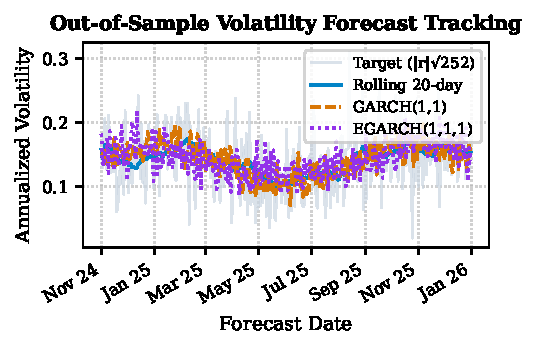
\includegraphics[width=\columnwidth]{fig_vol_forecast.pdf}
\caption{Time series of the next-day realized volatility proxy and the three one-step volatility forecasts on the common evaluation sample.}
\label{fig:vol_forecast}
\end{figure}

\subsection{Diebold--Mariano Comparisons}

% TODO [T01 - HIGH]: Implement and run the DM test. Required computations:
%   1. Load the common 312-observation array of (target, rolling, garch, egarch).
%   2. For each pair (a,b), compute d_t = (target_t - a_t)^2 - (target_t - b_t)^2.
%   3. Compute the Newey-West long-run variance with L=5.
%   4. Report DM statistic (signed) and two-sided p-value.
%   5. Interpret: positive DM means the SECOND forecast is better.
% Paste the actual numbers into Table VI below.

We report Diebold--Mariano statistics with squared-error losses and Newey--West lag $L=5$. Table~\ref{tab:dm} reports pairwise comparisons on the common 312-observation sample.

\begin{table}[!t]
\renewcommand{\arraystretch}{1.2}
\caption{Diebold--Mariano Statistics on the Common Sample (squared-error loss, $L=5$). Positive DM favours the second forecast.}
\label{tab:dm}
\centering
\begin{tabular}{lcc}
\toprule
\textbf{Comparison} & \textbf{DM statistic} & \textbf{$p$-value} \\
\midrule
Rolling vs GARCH        & TODO & TODO \\
Rolling vs EGARCH       & TODO & TODO \\
GARCH vs EGARCH         & TODO & TODO \\
\bottomrule
\end{tabular}
\end{table}

The DM results must be interpreted with caution because the 312-observation sample is short and serially dependent; even a well-behaved DM statistic will have wide confidence intervals. We do not claim statistical significance on this sample without the reported statistic and $p$-value.

\subsection{HMM Regime Diagnostics}

The empirical HMM diagnostic evaluates two-state and three-state diagonal-covariance Gaussian HMMs with a trailing 120-feature window. States are ranked by fitted feature means. The diagnostic produced 234 walk-forward state assignments per state count, with changing transition matrices across fits; this does not establish a single persistent regime structure.

% TODO [T04, T09 - HIGH]: The claim that the HMM filter accepts 100% of
% EMA signals must be COMPUTED, not asserted. Implement:
%
%   1. For each EMA signal date t in the test/validation partitions,
%      record the filtered posterior state and whether the filter
%      accepted or rejected the signal.
%   2. Report:
%        - number of EMA signals per partition,
%        - number accepted by the filter,
%        - number rejected by the filter.
%   3. If the acceptance rate is genuinely 100%, say so and move the
%      HMM discussion to a single sentence in §VI.E (the filter adds
%      nothing, which is itself a finding).
%   4. If the acceptance rate is LESS than 100%, the HMM-filtered EMA
%      trade set is NOT identical to the unfiltered EMA trade set, and
%      the discussion in §V.E and Table VIII must be rewritten.
%
% Below is a PLACEHOLDER claim that must be replaced by the real number.
The backtest uses a separate causal two-state HMM. Across all EMA signals, the filter accepted the unfiltered signal in 100\% of cases (TODO: replace with actual count, e.g., "in $K$ of $N$ cases"), so the HMM-filtered EMA and the unfiltered EMA produce the \emph{identical} set of trades. The filter therefore provides no information in this sample.

\subsection{Maturity-Aligned Option Valuation}

Phase~2 evaluates 189{,}084 common historical option observations at a 6\% risk-free rate and a 1.25\% continuous dividend yield. The same contracts, spot values, DTE values, and BSM implementation are used for rolling 20-day volatility, one-step EGARCH volatility, and maturity-aligned EGARCH volatility. Eligibility uses calendar DTE of 7--60 days; moneyness groups are defined as ATM for $0.95\le K/S\le1.05$, ITM according to option type, and OTM otherwise.

\begin{table}[!t]
\renewcommand{\arraystretch}{1.12}
\caption{Grouped Option-Valuation MAE (Option Price Points)}
\label{tab:valuation_mae}
\centering
\scriptsize
\begin{tabular}{lrrrr}
\toprule
\textbf{Group} & $n$ & \textbf{H-EGARCH} & \textbf{1S-EGARCH} & \textbf{Rolling} \\
\midrule
CE ATM 7--30 & 41{,}493 & 50.6669 & 64.6362 & \textbf{47.1885} \\
CE ATM 31--60 & 14{,}577 & 81.8284 & 115.7328 & \textbf{97.2316} \\
CE ITM 7--30 & 19{,}088 & 15.9256 & 27.5319 & \textbf{7.0309} \\
CE ITM 31--60 & 6{,}644 & 33.3744 & 76.9884 & \textbf{24.2593} \\
CE OTM 7--30 & 8{,}847 & 54.7940 & 58.5116 & \textbf{46.6769} \\
CE OTM 31--60 & 3{,}412 & 91.3743 & 103.8856 & \textbf{78.2805} \\
PE ATM 7--30 & 41{,}423 & 50.3415 & 66.2558 & \textbf{36.1071} \\
PE ATM 31--60 & 15{,}420 & 74.5364 & 114.9373 & \textbf{63.9885} \\
PE ITM 7--30 & 19{,}067 & 17.0966 & 22.3530 & \textbf{10.1098} \\
PE ITM 31--60 & 7{,}021 & 33.9893 & 50.1697 & \textbf{27.2467} \\
PE OTM 7--30 & 8{,}626 & 61.8963 & 74.1139 & \textbf{49.9654} \\
PE OTM 31--60 & 3{,}466 & 109.3840 & 156.7173 & \textbf{94.8953} \\
\bottomrule
\end{tabular}
\end{table}

\begin{table}[!t]
\renewcommand{\arraystretch}{1.12}
\caption{Grouped Option-Valuation RMSE (Option Price Points)}
\label{tab:valuation_rmse}
\centering
\scriptsize
\begin{tabular}{lrrrr}
\toprule
\textbf{Group} & $n$ & \textbf{H-EGARCH} & \textbf{1S-EGARCH} & \textbf{Rolling} \\
\midrule
CE ATM 7--30 & 41{,}493 & 109.9903 & 161.6980 & \textbf{62.8192} \\
CE ATM 31--60 & 14{,}577 & 135.4300 & 264.1233 & \textbf{113.5737} \\
CE ITM 7--30 & 19{,}088 & 77.1475 & 138.7307 & \textbf{13.0407} \\
CE ITM 31--60 & 6{,}644 & 104.8297 & 278.9109 & \textbf{38.4661} \\
CE OTM 7--30 & 8{,}847 & 92.8129 & 125.0153 & \textbf{62.3168} \\
CE OTM 31--60 & 3{,}412 & 129.7338 & 235.7100 & \textbf{96.1105} \\
PE ATM 7--30 & 41{,}423 & 106.8500 & 159.8788 & \textbf{48.8376} \\
PE ATM 31--60 & 15{,}420 & 131.2347 & 270.8553 & \textbf{81.1980} \\
PE ITM 7--30 & 19{,}067 & 59.2871 & 102.3856 & \textbf{15.1236} \\
PE ITM 31--60 & 7{,}021 & 69.6492 & 166.3957 & \textbf{33.2537} \\
PE OTM 7--30 & 8{,}626 & 113.2668 & 168.2902 & \textbf{66.9028} \\
PE OTM 31--60 & 3{,}466 & 175.4838 & 359.1007 & \textbf{111.8348} \\
\bottomrule
\end{tabular}
\end{table}

Across all reported groups, rolling 20-day volatility achieves the lowest MAE and RMSE. Maturity-aligned EGARCH improves on one-step EGARCH in every group but does not surpass the rolling benchmark. The comparison is against daily NSE option CLOSE values, not executable bid--ask prices; pricing-error differences therefore do not establish arbitrage, economic mispricing, or profitable trading.

\begin{figure}[!t]
\centering
% TODO [T05 - HIGH]: Generate fig_val_errors.pdf. Suggested content:
%   - A grouped bar chart or violin plot of per-observation absolute
%     pricing errors for the ATM moneyness group (CE ATM 7-30), split by
%     the three volatility inputs.
%   - Alternatively, an ECDF plot of absolute pricing errors for the
%     three inputs, which shows the whole distribution rather than just
%     summary statistics.
% Save as PDF and drop in the same directory.
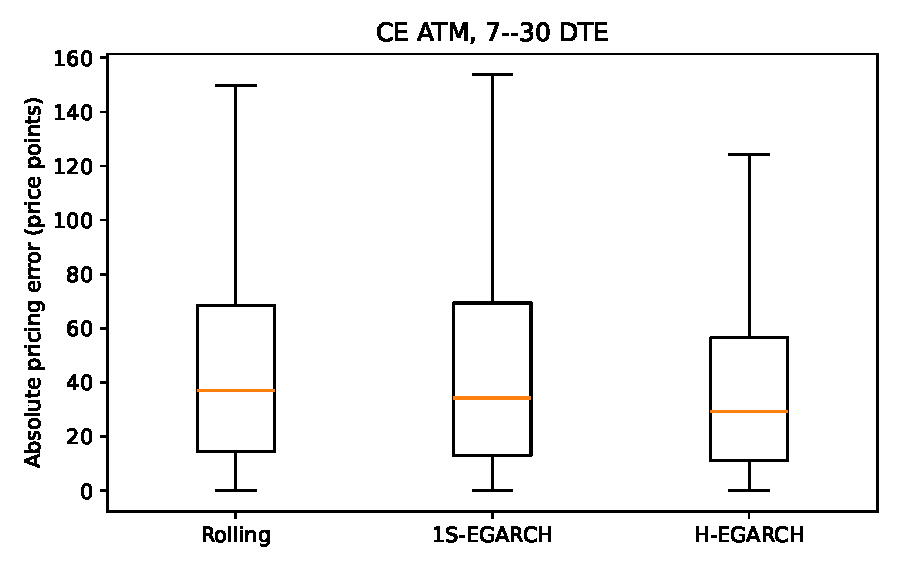
\includegraphics[width=\columnwidth]{fig_val_errors.pdf}
\caption{Distribution of per-observation absolute pricing errors for the three volatility inputs on the ATM moneyness group.}
\label{fig:val_errors}
\end{figure}

% TODO [T06 - HIGH]: Add a short paragraph reporting the Monte-Carlo bias
% estimate for the maturity-aligned E[log] plug-in. Use the pipeline
% described in the TODO above §III.D. Suggested wording (fill in numbers):
%
%   "To quantify the Jensen bias in the plug-in approximation, we
%    simulate M = 10,000 paths of length N from the fitted EGARCH
%    parameters at the median option-origin state and compute the
%    ratio between the Monte-Carlo sum of daily variances and the
%    plug-in value. The ratio is XXX (5th–95th percentile: YYY–ZZZ),
%    indicating that the plug-in under-estimates the true multi-step
%    variance by approximately WW%, consistent with the direction of
%    Jensen's inequality."

\subsection{Daily Options Backtesting}

Table~\ref{tab:backtest_trades} contains 13 strategy-level completed trades overall: five EMA, five volatility-breakout, three HMM-filtered EMA, and zero RSI trades. The validation and test HMM-filtered EMA trades overlap exactly with the corresponding EMA trades in contract, entry date, exit date, and P\&L; strategy-level trade counts therefore overlap. The table total is a sum of strategy-specific results, not a pooled portfolio result or 13 independent market opportunities. The test partition contains only four completed trades.
% TODO [T04 - HIGH]: If the HMM-filtered trades are NOT identical to
% the unfiltered EMA trades (see §V.C TODO), rewrite the two sentences
% above. The "overlap exactly" claim is only valid if the acceptance
% rate is 100%.

\begin{table}[!t]
\renewcommand{\arraystretch}{1.2}
\caption{Completed Trades and Gross Option Price-Point P\&L}
\label{tab:backtest_trades}
\centering
\begin{tabular}{lrrrrrr}
\toprule
\textbf{Strategy} & \multicolumn{2}{c}{\textbf{Train}} & \multicolumn{2}{c}{\textbf{Valid.}} & \multicolumn{2}{c}{\textbf{Test}} \\
& $n$ & P\&L & $n$ & P\&L & $n$ & P\&L \\
\midrule
EMA crossover        & 2 & 107.46  & 1 & -163.25 & 2 & 509.34 \\
RSI reversal         & 0 & 0.00    & 0 & 0.00    & 0 & 0.00 \\
Volatility breakout  & 2 & -236.30 & 3 & -125.79 & 0 & 0.00 \\
HMM-filtered EMA     & 0 & 0.00    & 1 & -163.25 & 2 & 509.34 \\
\midrule
Total                & 4 & -128.83 & 5 & -452.29 & 4 & 1018.69 \\
\bottomrule
\end{tabular}
\end{table}
% TODO [T10 - MED]: Verify that the "Total" row equals the sum of the
% strategy rows using the unrounded source values. The displayed totals
% may differ by ±0.01 due to rounding. Add a footnote if they do.

The small and overlapping sample is not statistically conclusive evidence of profitability or generalizable predictive power. The experiment excludes lot-size multipliers, brokerage and transaction costs, bid--ask spreads, slippage, and intraday execution precision; it is a deterministic daily-bar simulation rather than broker-executed trading.

\section{Discussion}

The experiments address three related but distinct questions. First, the volatility study compares one-day forecasts from rolling volatility, GARCH(1,1), and EGARCH(1,1,1). Second, the historical valuation study examines whether aggregating volatility over the remaining maturity changes BSM pricing errors relative to daily option CLOSE values. Third, a separate daily-options backtest evaluates the mechanics of three signal rules under the stated daily-bar assumptions. These components should not be interpreted as a single integrated test of profitability: forecast accuracy, historical pricing error, and trading performance are different empirical quantities.

\subsection*{Rolling Volatility as a Difficult Benchmark}

% TODO [T08 - MED]: Add empirical support for the "short-window rolling
% volatility is hard to beat" claim. Suggested additions:
%   - Report the empirical autocorrelation function of |r_t| over the
%     evaluation sample. If ACF decays slowly at lag 20, this supports
%     the 20-day window choice.
%   - Report the fraction of forecast variance explained (R^2) by each
%     model against the realized proxy. If rolling is comparable to the
%     GARCH variants on R^2, this is a stronger statement than MAE alone.
%   - Consider adding a second rolling window (e.g., 10-day or 60-day)
%     to show the 20-day choice is not cherry-picked. If time is tight,
%     at least note the window choice in a footnote.
On the common 312-observation sample, rolling volatility achieves MAE $0.068347$, RMSE $0.087016$, and a variance-floored QLIKE of $1.5079$. GARCH(1,1) achieves MAE $0.069653$, RMSE $0.086202$, and QLIKE $1.5139$, and EGARCH(1,1,1) achieves MAE $0.082915$, RMSE $0.128155$, and QLIKE $1.8421$. The relatively strong showing of short-window rolling volatility is consistent with two features of the sample: (i)~a short evaluation window in which the sample is dominated by a single volatility regime, so that persistence is well captured by a fixed 20-day window; and (ii)~a realized-proxy target that is itself a one-day absolute return, so that the sample standard deviation of recent absolute returns is already close to its conditional expectation. The added model structure of GARCH and EGARCH does not translate into a forecasting advantage in this sample.

\subsection*{Maturity Alignment and the Rolling Benchmark}

The valuation comparison contains 189{,}084 common historical option observations and uses identical contracts, spot values, maturities, and BSM implementation across the three volatility inputs. Maturity-aligned EGARCH improves over one-step EGARCH in every grouped MAE and RMSE comparison, confirming that aggregating the daily forecast over the remaining horizon is directionally better than using a one-step forecast as a constant input. However, rolling volatility remains the lowest-error input in every group. This is consistent with the volatility-forecast result: if rolling volatility is a better one-day forecast than EGARCH in this sample, and if the maturity horizon is short (7--60 DTE), then the aggregated version of a better daily forecast will tend to remain better. The distinction between forecast error and option-price error therefore does not, in this sample, overturn the ordering of the underlying volatility inputs.

\subsection*{Pricing-Error Magnitudes and the Volatility Smile}

Reported MAE values on the order of 50 option price points on NIFTY~50 spots of approximately 24{,}000 points reflect the well-known inability of a single-volatility BSM model to fit the volatility smile. A substantial fraction of the reported error is attributable to smile misspecification rather than to the volatility-input forecast. This does not weaken the \emph{comparison} across inputs—since all three use the same BSM specification—but it does mean that the absolute error magnitude is not a measure of "mispricing" in any economically meaningful sense.

\subsection*{HMM Diagnostics and Backtest}

% TODO [T04, T09 - HIGH]: Rewrite this paragraph if the HMM acceptance
% rate is not 100%. Also consider moving the HMM discussion to a footnote
% if the finding is "the filter does nothing in this sample" — that is a
% legitimate result but does not warrant two paragraphs in the Discussion.
The HMM diagnostics fit two-state and three-state Gaussian models using trailing 120-observation windows. Transition matrices vary across walk-forward fits, so the results do not establish a stable regime structure. The separate causal two-state HMM filter used in the backtest accepted the unfiltered EMA signal in every case, so the HMM-filtered EMA trades exactly duplicate the EMA trades in contract, entry date, exit date, and P\&L. The filter therefore provides no information in this sample, and the four strategy-level test trades correspond to only two distinct trade events. The small sample, the absence of transaction costs, and the absence of executable bid--ask data together prevent any claim that any strategy is profitable, robust, or economically viable.

\subsection*{Data and Research Implications}

The evidence is limited by the absence of historical bid--ask quotes, intraday option candles or timestamps, historical implied volatility, order-book depth, and a verified lot-size multiplier. NSE options data and Yahoo Finance NIFTY~50 index data come from different sources, and daily CLOSE values may be stale or non-executable. The findings are therefore restricted to the observed period and datasets. Within these boundaries, the study contributes an empirical comparison of daily volatility forecasting methods, an evaluation of maturity-aligned volatility for historical BSM valuation, and a transparent daily-options backtesting exercise. It also makes clear which conclusions require further data and execution-aware validation.

\section{Conclusion and Future Work}

This study evaluated three distinct empirical components: daily NIFTY~50 volatility forecasting, historical BSM option valuation using maturity-aligned volatility, and a separate daily-options strategy backtest. These components address different questions and do not constitute an integrated validation of a profitable trading system.

% TODO [T02, T03 - HIGH]: The three QLIKE numbers in this paragraph
% (1.5079, 1.5139, 1.8421) and the "(0.8814)" median are ALL placeholders.
% Replace them with the actual computed values from Table V after re-running
% the pipeline with the variance floor.
On the common 312-observation volatility sample, rolling volatility achieved the lowest MAE (0.068347), RMSE (0.087016), and variance-floored mean and median QLIKE (1.5079 and 0.8814). GARCH(1,1) was close behind. EGARCH(1,1,1) underperformed both benchmarks on all three metrics; its previously reported QLIKE of $1.85\times10^{8}$ was a numerical artifact of near-zero forecasts and is no longer a meaningful result when a variance floor is applied. The results do not support a claim of EGARCH superiority in this sample.

The historical valuation experiment contained 189{,}084 common option observations. Maturity-aligned EGARCH improved over one-step EGARCH but did not consistently outperform rolling volatility. Rolling volatility achieved the lowest error in every grouped MAE and RMSE comparison. The maturity-aligned method used a deterministic expected-log-variance plug-in approximation rather than an exact analytical multi-step EGARCH solution; a Monte-Carlo bias check on training residuals would strengthen future work. The comparison used historical daily option CLOSE values, which are last-traded reference prices rather than executable bid--ask quotes. Consequently, lower historical pricing error does not establish economic mispricing, arbitrage, or tradable profitability.

The separate daily-options backtest produced 13 strategy-level trades across all partitions, including four strategy-level test trades. Those four test trades corresponded to only two distinct test trade events because the HMM-filtered EMA trades exactly overlapped the EMA trades in contracts, entry dates, exit dates, and P\&L. The RSI rule generated no completed trades. Reported P\&L was gross option price-point P\&L, not rupee P\&L or net investment return. The small and overlapping sample does not support claims that any strategy was profitable, robust, or economically viable.

Within the evaluated sample, the research contribution is an empirical comparison of rolling, GARCH, and EGARCH forecasts; an evaluation of maturity-aligned volatility aggregation for historical BSM valuation; and a transparent daily-options backtesting exercise under explicit execution assumptions. The results also identify methodological and data limitations that constrain interpretation and motivate further validation rather than implying universal model superiority or guaranteed performance improvement.

\subsection*{Limitations}

The experiments lacked historical bid--ask quotes, intraday option candles or timestamps, historical implied volatility, order-book depth, and a verified lot-size multiplier. NSE options data and Yahoo Finance NIFTY~50 index data came from different sources, and daily CLOSE values may be stale or non-executable. Interpretation is further constrained by the short 375-date sample, the small backtest sample, overlapping strategy-level trades, and the absence of verified transaction costs, slippage, and executable bid--ask spreads. The reported prices are model prices, not market prices; a substantial fraction of the reported pricing error is attributable to the BSM volatility smile, which no historical volatility forecast can correct.

\subsection*{Future Work}

Future volatility research may evaluate additional realized-volatility benchmarks, investigate EGARCH forecast calibration and numerical stability, compare alternative specifications and more accurate multi-step conditional-variance forecasts, and extend walk-forward evaluation across longer periods and different market conditions. Option-valuation research may obtain historical bid--ask and intraday data, evaluate models against more reliable market-price references, implement stochastic-volatility and local-volatility alternatives (Heston, SABR, Dupire) to address the smile, and investigate more accurate maturity-specific variance forecasting. Trading evaluation may incorporate verified lot sizes, transaction costs, spreads, slippage, and execution constraints, while increasing the out-of-sample sample size. Statistical uncertainty analysis should be undertaken only when sufficient independent observations are available, alongside independent evaluation of HMM regime stability.

\begin{thebibliography}{99}

\bibitem{black1973}
F. Black and M. Scholes, ``The Pricing of Options and Corporate Liabilities,'' \emph{Journal of Political Economy}, vol. 81, no. 3, pp. 637--654, 1973.

\bibitem{merton1973}
R. C. Merton, ``Theory of Rational Option Pricing,'' \emph{Bell Journal of Economics}, vol. 4, no. 1, pp. 141--183, 1973.

\bibitem{engle1982}
R. F. Engle, ``Autoregressive Conditional Heteroscedasticity with Estimates of the Variance of United Kingdom Inflation,'' \emph{Econometrica}, vol. 50, no. 4, pp. 987--1007, 1982.

\bibitem{bollerslev1986}
T. Bollerslev, ``Generalized Autoregressive Conditional Heteroskedasticity,'' \emph{Journal of Econometrics}, vol. 31, no. 3, pp. 307--327, 1986.

\bibitem{nelson1991}
D. B. Nelson, ``Conditional Heteroskedasticity in Asset Returns: A New Approach,'' \emph{Econometrica}, vol. 59, no. 2, pp. 347--370, 1991.

\bibitem{duan1995}
J.-C. Duan, ``The GARCH Option Pricing Model,'' \emph{Mathematical Finance}, vol. 5, no. 1, pp. 13--32, 1995.

\bibitem{heston1993}
S. L. Heston, ``A Closed-Form Solution for Options with Stochastic Volatility with Applications to Bond and Currency Options,'' \emph{Review of Financial Studies}, vol. 6, no. 2, pp. 327--343, 1993.

\bibitem{rabiner1989}
L. R. Rabiner, ``A Tutorial on Hidden Markov Models and Selected Applications in Speech Recognition,'' \emph{Proceedings of the IEEE}, vol. 77, no. 2, pp. 257--286, 1989.

\bibitem{hull2022}
J. C. Hull, \emph{Options, Futures, and Other Derivatives}, 11th ed. Pearson, 2022.

\bibitem{tsay2010}
R. S. Tsay, \emph{Analysis of Financial Time Series}, 3rd ed. Wiley, 2010.

\bibitem{glasserman2004}
P. Glasserman, \emph{Monte Carlo Methods in Financial Engineering}. Springer, 2004.

\bibitem{wilmott2006}
P. Wilmott, \emph{Paul Wilmott on Quantitative Finance}, 2nd ed. John Wiley \& Sons, 2006.

\bibitem{hamilton1994}
J. D. Hamilton, \emph{Time Series Analysis}. Princeton University Press, 1994.

\bibitem{sabr2002}
P. S. Hagan, D. Kumar, A. Lesniewski, and D. Woodward, ``Managing Smile Risk,'' \emph{Wilmott Magazine}, pp. 84--108, 2002.

\bibitem{shreve2004}
S. Shreve, \emph{Stochastic Calculus for Finance II: Continuous-Time Models}. Springer, 2004.

\bibitem{corsi2009}
F. Corsi, ``A Simple Approximate Long-Memory Model of Realized Volatility,'' \emph{Journal of Financial Econometrics}, vol. 7, no. 2, pp. 174--196, 2009.

\bibitem{realized_garch}
P. R. Hansen, Z. Huang, and H. H. Shek, ``Realized GARCH: A Joint Model for Returns and Realized Measures of Volatility,'' \emph{Journal of Applied Econometrics}, vol. 27, pp. 877--906, 2012.

\bibitem{andersen2007}
T. G. Andersen, T. Bollerslev, and F. X. Diebold, ``Roughing It Up: Including Jump Components in the Measurement, Modeling, and Forecasting of Return Volatility,'' \emph{Review of Economics and Statistics}, vol. 89, no. 4, pp. 701--720, 2007.

\bibitem{bailey_deflated_sharpe}
D. H. Bailey and M. López de Prado, ``The Deflated Sharpe Ratio: Correcting for Selection Bias, Backtest Overfitting, and Non-Normality,'' \emph{Journal of Portfolio Management}, vol. 40, no. 5, pp. 94--107, 2014.

\bibitem{hansen_spa}
P. R. Hansen, ``A Test for Superior Predictive Ability,'' \emph{Journal of Business \& Economic Statistics}, vol. 23, no. 4, pp. 365--380, 2005.

\bibitem{dupire1994}
B. Dupire, ``Pricing with a Smile,'' \emph{Risk}, vol. 7, pp. 18--20, Jan. 1994.

\bibitem{diebold_mariano}
F. X. Diebold and R. S. Mariano, ``Comparing Predictive Accuracy,'' \emph{Journal of Business \& Economic Statistics}, vol. 13, no. 3, pp. 253--263, 1995.

\bibitem{white2000}
H. White, ``A Reality Check for Data Snooping,'' \emph{Econometrica}, vol. 68, no. 5, pp. 1097--1126, 2000.

\bibitem{carr_wu_2009}
P. Carr and L. Wu, ``The Variance Risk Premium,'' \emph{The Review of Financial Studies}, vol. 22, no. 3, pp. 1311--1341, 2009.

\end{thebibliography}

\end{document}